\documentclass[10pt]{article}

\usepackage[margin=1.8cm]{geometry}
\usepackage{amsmath,amssymb}
\usepackage{tikz}
\usetikzlibrary{arrows.meta,positioning,calc,fit,backgrounds}
\usepackage{booktabs}
\usepackage{array}
\usepackage{longtable}
\usepackage{multicol}
\usepackage{enumitem}
\usepackage{xcolor}
\usepackage{listings}
\usepackage{hyperref}
\usepackage{parskip}
\usepackage{colortbl}

\hypersetup{colorlinks=true, linkcolor=blue!50!black, urlcolor=blue!50!black}

\lstset{basicstyle=\ttfamily\small, showstringspaces=false, columns=fullflexible}

\newcommand{\op}[1]{\texttt{#1}}
\definecolor{hdrbg}{HTML}{2B3A55}
\newcommand{\grouphead}[1]{\rowcolor{hdrbg!12}\multicolumn{5}{l}{\textbf{#1}}\\}

\title{\bfseries MIPS Reference Data\\[2pt]\large A More Readable Edition}
\author{Reformatted from the Patterson \& Hennessy MIPS ``Green Card''\\
\emph{Computer Organization and Design}, 4th ed., \textcopyright\ 2009 Elsevier}
\date{}

\begin{document}
\maketitle
\tableofcontents
\newpage

% ==========================================================================
\section{How to Use This Sheet}

This is the same reference data as the original MIPS ``green card,'' but
reorganized and enlarged for readability:
\begin{itemize}
  \item Instructions are grouped \textbf{by category} (arithmetic, logical,
  data transfer, branch/jump, comparison, floating point) instead of strict
  alphabetical order.
  \item Every table uses a font large enough to read without a magnifying
  glass.
  \item Field/bit diagrams (instruction formats, stack frame, memory map,
  exception registers) are redrawn as clean boxes.
\end{itemize}

Common notation used in the ``Operation'' column:
\begin{center}
\begin{tabular}{@{}ll@{}}
\toprule
Notation & Meaning \\
\midrule
\op{R[rs]}, \op{R[rt]}, \op{R[rd]} & value in the named general-purpose register \\
\op{M[addr]} & value in memory at address \op{addr} \\
\op{F[fs]}, \op{F[ft]}, \op{F[fd]} & value in the named floating-point register \\
\op{SignExtImm} & 16-bit immediate, sign-extended to 32 bits \\
\op{ZeroExtImm} & 16-bit immediate, zero-extended to 32 bits \\
\op{PC} & program counter \\
\op{Hi}, \op{Lo} & the two special multiply/divide result registers \\
\bottomrule
\end{tabular}
\end{center}

% ==========================================================================
\section{Instruction Formats}

Every MIPS instruction is 32 bits, in one of five layouts:

\begin{center}
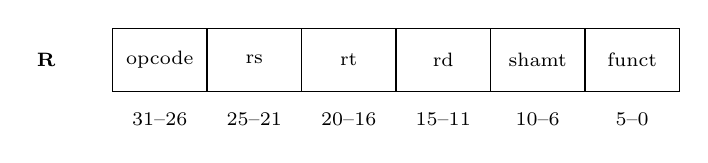
\begin{tikzpicture}[font=\scriptsize]
  \newcommand{\field}[3]{\draw (#1,0) rectangle ++(#2,0.8) node[midway]{#3};}
  % R
  \node[left] at (-0.6,0.4) {\textbf{R}};
  \field{0}{1.2}{opcode} \field{1.2}{1.2}{rs} \field{2.4}{1.2}{rt}
  \field{3.6}{1.2}{rd} \field{4.8}{1.2}{shamt} \field{6.0}{1.2}{funct}
  \node[below] at (0.6,-0.15) {\scriptsize 31--26};
  \node[below] at (1.8,-0.15) {\scriptsize 25--21};
  \node[below] at (3.0,-0.15) {\scriptsize 20--16};
  \node[below] at (4.2,-0.15) {\scriptsize 15--11};
  \node[below] at (5.4,-0.15) {\scriptsize 10--6};
  \node[below] at (6.6,-0.15) {\scriptsize 5--0};
\end{tikzpicture}

\vspace{0.5cm}
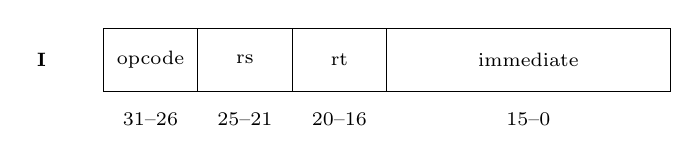
\begin{tikzpicture}[font=\scriptsize]
  \newcommand{\field}[3]{\draw (#1,0) rectangle ++(#2,0.8) node[midway]{#3};}
  % I
  \node[left] at (-0.6,0.4) {\textbf{I}};
  \field{0}{1.2}{opcode} \field{1.2}{1.2}{rs} \field{2.4}{1.2}{rt}
  \field{3.6}{3.6}{immediate}
  \node[below] at (0.6,-0.15) {\scriptsize 31--26};
  \node[below] at (1.8,-0.15) {\scriptsize 25--21};
  \node[below] at (3.0,-0.15) {\scriptsize 20--16};
  \node[below] at (5.4,-0.15) {\scriptsize 15--0};
\end{tikzpicture}

\vspace{0.5cm}
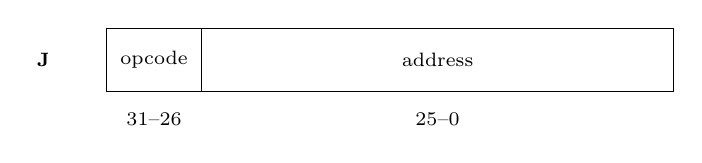
\begin{tikzpicture}[font=\scriptsize]
  \newcommand{\field}[3]{\draw (#1,0) rectangle ++(#2,0.8) node[midway]{#3};}
  % J
  \node[left] at (-0.6,0.4) {\textbf{J}};
  \field{0}{1.2}{opcode} \field{1.2}{6.0}{address}
  \node[below] at (0.6,-0.15) {\scriptsize 31--26};
  \node[below] at (4.2,-0.15) {\scriptsize 25--0};
\end{tikzpicture}

\vspace{0.5cm}
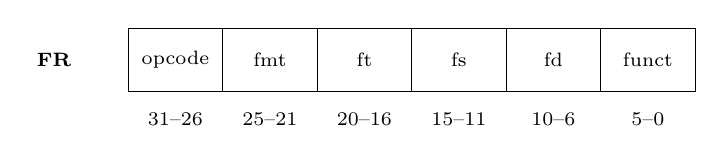
\begin{tikzpicture}[font=\scriptsize]
  \newcommand{\field}[3]{\draw (#1,0) rectangle ++(#2,0.8) node[midway]{#3};}
  % FR
  \node[left] at (-0.6,0.4) {\textbf{FR}};
  \field{0}{1.2}{opcode} \field{1.2}{1.2}{fmt} \field{2.4}{1.2}{ft}
  \field{3.6}{1.2}{fs} \field{4.8}{1.2}{fd} \field{6.0}{1.2}{funct}
  \node[below] at (0.6,-0.15) {\scriptsize 31--26};
  \node[below] at (1.8,-0.15) {\scriptsize 25--21};
  \node[below] at (3.0,-0.15) {\scriptsize 20--16};
  \node[below] at (4.2,-0.15) {\scriptsize 15--11};
  \node[below] at (5.4,-0.15) {\scriptsize 10--6};
  \node[below] at (6.6,-0.15) {\scriptsize 5--0};
\end{tikzpicture}

\vspace{0.5cm}
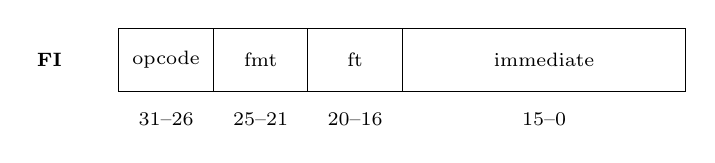
\begin{tikzpicture}[font=\scriptsize]
  \newcommand{\field}[3]{\draw (#1,0) rectangle ++(#2,0.8) node[midway]{#3};}
  % FI
  \node[left] at (-0.6,0.4) {\textbf{FI}};
  \field{0}{1.2}{opcode} \field{1.2}{1.2}{fmt} \field{2.4}{1.2}{ft}
  \field{3.6}{3.6}{immediate}
  \node[below] at (0.6,-0.15) {\scriptsize 31--26};
  \node[below] at (1.8,-0.15) {\scriptsize 25--21};
  \node[below] at (3.0,-0.15) {\scriptsize 20--16};
  \node[below] at (5.4,-0.15) {\scriptsize 15--0};
\end{tikzpicture}
\end{center}

% ==========================================================================
\section{Core Integer Instruction Set}

Format legend: \textbf{R} = register, \textbf{I} = immediate, \textbf{J} =
jump. The last column gives \op{opcode/funct} in hex (``\op{0/20}'' means
opcode \op{0} with \op{funct} field \op{0x20}; a bare hex value is the
opcode alone, used when there is no funct field).

\subsection{Arithmetic}
\begin{center}
\small
\begin{tabular}{@{}p{2.7cm}p{1.6cm}cp{5.4cm}l@{}}
\toprule
Name & Mnemonic & Fmt & Operation & Opcode/Funct \\
\midrule
Add                 & \op{add}  & R & \op{R[rd] = R[rs] + R[rt]} & \op{0/20} \\
Add Immediate       & \op{addi} & I & \op{R[rt] = R[rs] + SignExtImm} & \op{8} \\
Add Unsigned        & \op{addu} & R & \op{R[rd] = R[rs] + R[rt]} & \op{0/21} \\
Add Imm.\ Unsigned  & \op{addiu}& I & \op{R[rt] = R[rs] + SignExtImm} & \op{9} \\
Subtract            & \op{sub}  & R & \op{R[rd] = R[rs] -- R[rt]} & \op{0/22} \\
Subtract Unsigned   & \op{subu} & R & \op{R[rd] = R[rs] -- R[rt]} & \op{0/23} \\
Multiply            & \op{mult} & R & \op{\{Hi,Lo\} = R[rs] * R[rt]} & \op{0/18} \\
Multiply Unsigned   & \op{multu}& R & \op{\{Hi,Lo\} = R[rs] * R[rt]} & \op{0/19} \\
Divide              & \op{div}  & R & \op{Lo=R[rs]/R[rt]; Hi=R[rs]\%R[rt]} & \op{0/1a} \\
Divide Unsigned     & \op{divu} & R & \op{Lo=R[rs]/R[rt]; Hi=R[rs]\%R[rt]} & \op{0/1b} \\
Move From Hi        & \op{mfhi} & R & \op{R[rd] = Hi} & \op{0/10} \\
Move From Lo        & \op{mflo} & R & \op{R[rd] = Lo} & \op{0/12} \\
\bottomrule
\end{tabular}
\end{center}
\emph{Add, Add Immediate and Subtract may cause an overflow exception;
their Unsigned counterparts never do.}

\subsection{Logical \& Shift}
\begin{center}
\small
\begin{tabular}{@{}p{2.7cm}p{1.6cm}cp{5.4cm}l@{}}
\toprule
Name & Mnemonic & Fmt & Operation & Opcode/Funct \\
\midrule
And              & \op{and}  & R & \op{R[rd] = R[rs] \& R[rt]} & \op{0/24} \\
And Immediate    & \op{andi} & I & \op{R[rt] = R[rs] \& ZeroExtImm} & \op{c} \\
Or               & \op{or}   & R & \op{R[rd] = R[rs] | R[rt]} & \op{0/25} \\
Or Immediate     & \op{ori}  & I & \op{R[rt] = R[rs] | ZeroExtImm} & \op{d} \\
Nor              & \op{nor}  & R & \op{R[rd] = \textasciitilde(R[rs] | R[rt])} & \op{0/27} \\
Shift Left Logical  & \op{sll} & R & \op{R[rd] = R[rt] \textless\textless shamt} & \op{0/00} \\
Shift Right Logical & \op{srl} & R & \op{R[rd] = R[rt] \textgreater\textgreater shamt} & \op{0/02} \\
Shift Right Arithmetic & \op{sra} & R & \op{R[rd] = R[rt] \textgreater\textgreater\textgreater shamt} & \op{0/03} \\
\bottomrule
\end{tabular}
\end{center}

\subsection{Data Transfer (Load / Store)}
\begin{center}
\small
\begin{tabular}{@{}p{2.9cm}p{1.6cm}cp{6.3cm}l@{}}
\toprule
Name & Mnemonic & Fmt & Operation & Opcode \\
\midrule
Load Word           & \op{lw}  & I & \op{R[rt] = M[R[rs]+SignExtImm]} & \op{23} \\
Store Word          & \op{sw}  & I & \op{M[R[rs]+SignExtImm] = R[rt]} & \op{2b} \\
Load Byte Unsigned  & \op{lbu} & I & \op{R[rt] = \{24'b0, M[R[rs]+SignExtImm](7:0)\}} & \op{24} \\
Store Byte          & \op{sb}  & I & \op{M[R[rs]+SignExtImm](7:0) = R[rt](7:0)} & \op{28} \\
Load Halfword Unsigned & \op{lhu} & I & \op{R[rt] = \{16'b0, M[R[rs]+SignExtImm](15:0)\}} & \op{25} \\
Store Halfword      & \op{sh}  & I & \op{M[R[rs]+SignExtImm](15:0) = R[rt](15:0)} & \op{29} \\
Load Upper Immediate& \op{lui} & I & \op{R[rt] = \{immediate, 16'b0\}} & \op{f} \\
Load Linked         & \op{ll}  & I & \op{R[rt] = M[R[rs]+SignExtImm]} & \op{30} \\
Store Conditional   & \op{sc}  & I & \op{M[..]=R[rt]; R[rt] = (atomic)?1:0} & \op{38} \\
\bottomrule
\end{tabular}
\end{center}
\emph{\op{ll}/\op{sc} form an atomic test-and-set pair: \op{sc} stores its
value and returns 1 in \op{R[rt]} only if the memory word has not been
touched since the matching \op{ll}; otherwise it fails and returns 0.}

\subsection{Comparison}
\begin{center}
\small
\begin{tabular}{@{}p{3.1cm}p{1.6cm}cp{6.1cm}l@{}}
\toprule
Name & Mnemonic & Fmt & Operation & Opcode/Funct \\
\midrule
Set Less Than             & \op{slt}   & R & \op{R[rd] = (R[rs]\textless R[rt]) ? 1 : 0} & \op{0/2a} \\
Set Less Than Immediate   & \op{slti}  & I & \op{R[rt] = (R[rs]\textless SignExtImm) ? 1:0} & \op{a} \\
Set Less Than Unsigned    & \op{sltu}  & R & \op{R[rd] = (R[rs]\textless R[rt]) ? 1:0} (unsigned) & \op{0/2b} \\
Set Less Than Imm.\ Unsigned & \op{sltiu} & I & \op{R[rt] = (R[rs]\textless SignExtImm) ? 1:0} (unsigned) & \op{b} \\
\bottomrule
\end{tabular}
\end{center}

\subsection{Branch \& Jump}
\begin{center}
\small
\begin{tabular}{@{}p{3.1cm}p{1.6cm}cp{6.1cm}l@{}}
\toprule
Name & Mnemonic & Fmt & Operation & Opcode \\
\midrule
Branch On Equal     & \op{beq} & I & \op{if(R[rs]==R[rt]) PC=PC+4+BranchAddr} & \op{4} \\
Branch On Not Equal & \op{bne} & I & \op{if(R[rs]!=R[rt]) PC=PC+4+BranchAddr} & \op{5} \\
Jump                & \op{j}   & J & \op{PC = JumpAddr} & \op{2} \\
Jump And Link       & \op{jal} & J & \op{R[31]=PC+8; PC=JumpAddr} & \op{3} \\
Jump Register       & \op{jr}  & R & \op{PC = R[rs]} & \op{0/08} \\
\bottomrule
\end{tabular}
\end{center}

\subsection{Field-encoding notes (from the original card)}
\begin{enumerate}[label=(\arabic*)]
  \item May cause overflow exception.
  \item \op{SignExtImm = \{ 16\{immediate[15]\}, immediate \}}
  \item \op{ZeroExtImm = \{ 16\{1b'0\}, immediate \}}
  \item \op{BranchAddr = \{ 14\{immediate[15]\}, immediate, 2'b0 \}}
  \item \op{JumpAddr = \{ PC+4[31:28], address, 2'b0 \}}
  \item Operands considered unsigned numbers (vs.\ 2's complement).
  \item Atomic test\&set pair; \op{R[rt] = 1} if pair atomic, 0 if not
  atomic.
\end{enumerate}

% ==========================================================================
\section{Floating-Point Instruction Set}

Formats \textbf{FR}/\textbf{FI} mirror R/I but with floating-point register
fields \op{fmt} (single \op{s}=\op{10}$_{16}$ / double \op{d}=\op{11}$_{16}$),
\op{ft}, \op{fs}, \op{fd}. Opcode/Funct column shows \op{opcode/fmt/funct}.

\subsection{Arithmetic}
\begin{center}
\small
\begin{tabular}{@{}p{3.0cm}p{1.3cm}cp{6.4cm}l@{}}
\toprule
Name & Mnemonic & Fmt & Operation & Opcode/Fmt/Funct \\
\midrule
FP Add Single      & \op{add.s} & FR & \op{F[fd] = F[fs] + F[ft]} & \op{11/10/0} \\
FP Add Double       & \op{add.d} & FR & \op{\{F[fd],F[fd+1]\} = \{F[fs],F[fs+1]\}+\{F[ft],F[ft+1]\}} & \op{11/11/0} \\
FP Subtract Single & \op{sub.s} & FR & \op{F[fd] = F[fs] -- F[ft]} & \op{11/10/1} \\
FP Subtract Double  & \op{sub.d} & FR & \op{\{F[fd],F[fd+1]\} = \{F[fs],F[fs+1]\}-\{F[ft],F[ft+1]\}} & \op{11/11/1} \\
FP Multiply Single & \op{mul.s} & FR & \op{F[fd] = F[fs] * F[ft]} & \op{11/10/2} \\
FP Multiply Double  & \op{mul.d} & FR & \op{\{F[fd],F[fd+1]\} = \{F[fs],F[fs+1]\}*\{F[ft],F[ft+1]\}} & \op{11/11/2} \\
FP Divide Single   & \op{div.s} & FR & \op{F[fd] = F[fs] / F[ft]} & \op{11/10/3} \\
FP Divide Double     & \op{div.d} & FR & \op{\{F[fd],F[fd+1]\} = \{F[fs],F[fs+1]\}/\{F[ft],F[ft+1]\}} & \op{11/11/3} \\
\bottomrule
\end{tabular}
\end{center}

\subsection{Compare \& Branch}
\begin{center}
\small
\begin{tabular}{@{}p{3.0cm}p{1.6cm}cp{6.1cm}l@{}}
\toprule
Name & Mnemonic & Fmt & Operation & Opcode/Fmt/Funct \\
\midrule
FP Compare Single & \op{c.$x$.s}* & FR & \op{FPcond = (F[fs] op F[ft]) ? 1:0} & \op{11/10/$y$} \\
FP Compare Double  & \op{c.$x$.d}* & FR & \op{FPcond = (\{F[fs],F[fs{+}1]\} op \{F[ft],F[ft{+}1]\}) ? 1:0} & \op{11/11/$y$} \\
Branch On FP True  & \op{bc1t}  & FI & \op{if(FPcond) PC=PC+4+BranchAddr} & \op{11/8/1} \\
Branch On FP False & \op{bc1f}  & FI & \op{if(!FPcond) PC=PC+4+BranchAddr} & \op{11/8/0} \\
\bottomrule
\end{tabular}
\end{center}
\emph{* $x$ is \op{eq}, \op{lt}, or \op{le}; $op$ is \op{==}, \op{\textless},
or \op{\textless=}; $y$ is \op{32}, \op{3c}, or \op{3e} respectively.}

\subsection{Data Transfer \& Misc.}
\begin{center}
\small
\begin{tabular}{@{}p{3.0cm}p{1.6cm}cp{6.1cm}l@{}}
\toprule
Name & Mnemonic & Fmt & Operation & Opcode \\
\midrule
Load FP Single  & \op{lwc1} & I & \op{F[rt] = M[R[rs]+SignExtImm]} & \op{31} \\
Store FP Single & \op{swc1} & I & \op{M[R[rs]+SignExtImm] = F[rt]} & \op{39} \\
Load FP Double   & \op{ldc1} & I & \op{F[rt]=M[..]; F[rt+1]=M[..+4]} & \op{35} \\
Store FP Double  & \op{sdc1} & I & \op{M[..]=F[rt]; M[..+4]=F[rt+1]} & \op{3d} \\
Move From Control & \op{mfc0} & R & \op{R[rd] = CR[rs]} & \op{10/0/0} \\
\bottomrule
\end{tabular}
\end{center}

% ==========================================================================
\section{Pseudoinstructions}
Convenience instructions the assembler expands into one or more real
instructions.

\begin{center}
\begin{tabular}{@{}p{4.6cm}lp{6.5cm}@{}}
\toprule
Name & Mnemonic & Operation \\
\midrule
Branch Less Than            & \op{blt} & \op{if(R[rs]\textless R[rt]) PC = Label} \\
Branch Greater Than         & \op{bgt} & \op{if(R[rs]\textgreater R[rt]) PC = Label} \\
Branch Less Than or Equal   & \op{ble} & \op{if(R[rs]\textless=R[rt]) PC = Label} \\
Branch Greater Than or Equal& \op{bge} & \op{if(R[rs]\textgreater=R[rt]) PC = Label} \\
Load Immediate              & \op{li}  & \op{R[rd] = immediate} \\
Move                        & \op{move}& \op{R[rd] = R[rs]} \\
\bottomrule
\end{tabular}
\end{center}

% ==========================================================================
\section{Registers}

\subsection{Register name, number, use, call convention}
\begin{center}
\begin{tabular}{@{}lcp{6.3cm}c@{}}
\toprule
Name & Number & Use & Preserved across a call? \\
\midrule
\op{\$zero}     & 0     & The constant value 0            & n/a \\
\op{\$at}       & 1     & Assembler temporary              & No \\
\op{\$v0--\$v1} & 2--3  & Function results, expression eval & No \\
\op{\$a0--\$a3} & 4--7  & Arguments                         & No \\
\op{\$t0--\$t7} & 8--15 & Temporaries                       & No \\
\op{\$s0--\$s7} & 16--23& Saved temporaries                 & Yes \\
\op{\$t8--\$t9} & 24--25& Temporaries                       & No \\
\op{\$k0--\$k1} & 26--27& Reserved for OS kernel             & No \\
\op{\$gp}       & 28    & Global pointer                    & Yes \\
\op{\$sp}       & 29    & Stack pointer                     & Yes \\
\op{\$fp}       & 30    & Frame pointer                     & Yes \\
\op{\$ra}       & 31    & Return address                    & Yes \\
\bottomrule
\end{tabular}
\end{center}

\subsection{Memory map and stack frame}
\begin{center}
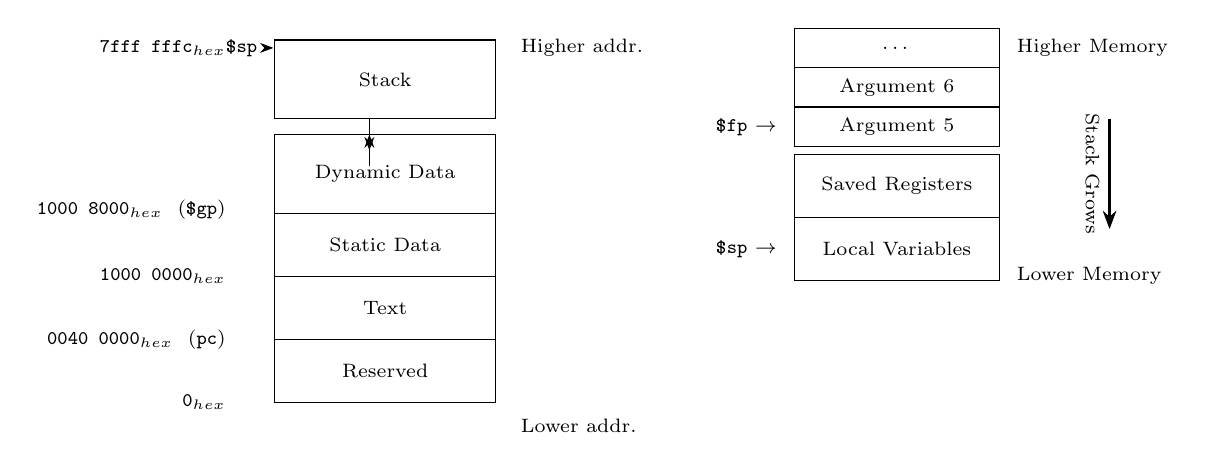
\begin{tikzpicture}[font=\scriptsize,>=Stealth]
  % Memory allocation
  \node[draw,minimum width=2.8cm,minimum height=1.0cm] (stack) at (0,4.5) {Stack};
  \node[draw,minimum width=2.8cm,minimum height=1.0cm] (dyn)   at (0,3.3) {Dynamic Data};
  \node[draw,minimum width=2.8cm,minimum height=0.8cm] (stat)  at (0,2.4) {Static Data};
  \node[draw,minimum width=2.8cm,minimum height=0.8cm] (text)  at (0,1.6) {Text};
  \node[draw,minimum width=2.8cm,minimum height=0.8cm] (res)   at (0,0.8) {Reserved};
  \draw[->] (-0.2,4.0) -- (-0.2,3.6);
  \draw[->] (-0.2,3.4) -- (-0.2,3.8);
  \node[left] at (-1.5,4.9) {\op{\$sp}};
  \draw[->] (-1.5,4.9) -- (-1.42,4.9);
  \node[left] at (-1.55,4.9) {};
  \node[left] at (-1.9,4.9) {\op{7fff fffc}$_{hex}$};
  \node[left] at (-1.9,2.85) {\op{1000 8000}$_{hex}$ \ (\op{\$gp})};
  \node[left] at (-1.9,2.0) {\op{1000 0000}$_{hex}$};
  \node[left] at (-1.9,1.2) {\op{0040 0000}$_{hex}$ \ (\op{pc})};
  \node[left] at (-1.9,0.4) {\op{0}$_{hex}$};
  \node[right] at (1.6,4.9) {Higher addr.};
  \node[right] at (1.6,0.1) {Lower addr.};

  % Stack frame
  \node[draw,minimum width=2.6cm,minimum height=0.5cm] (dots) at (6.5,4.9) {\dots};
  \node[draw,minimum width=2.6cm,minimum height=0.5cm] (a6) at (6.5,4.4) {Argument 6};
  \node[draw,minimum width=2.6cm,minimum height=0.5cm] (a5) at (6.5,3.9) {Argument 5};
  \node[draw,minimum width=2.6cm,minimum height=0.8cm] (sr) at (6.5,3.15) {Saved Registers};
  \node[draw,minimum width=2.6cm,minimum height=0.8cm] (lv) at (6.5,2.35) {Local Variables};
  \node[left] at (5.1,3.9) {\op{\$fp} $\to$};
  \node[left] at (5.1,2.35) {\op{\$sp} $\to$};
  \node[right] at (7.9,4.9) {Higher Memory};
  \node[right] at (7.9,2.0) {Lower Memory};
  \draw[->,thick] (9.2,4.0) -- (9.2,2.6) node[midway,right,rotate=-90,anchor=north]{Stack Grows};
\end{tikzpicture}
\end{center}

% ==========================================================================
\section{Data Sizes, Alignment \& Number Formats}

\subsection{Data alignment}
A word begins at an address divisible by 4; a halfword at an address
divisible by 2. MIPS is \textbf{big-endian}.
\begin{center}
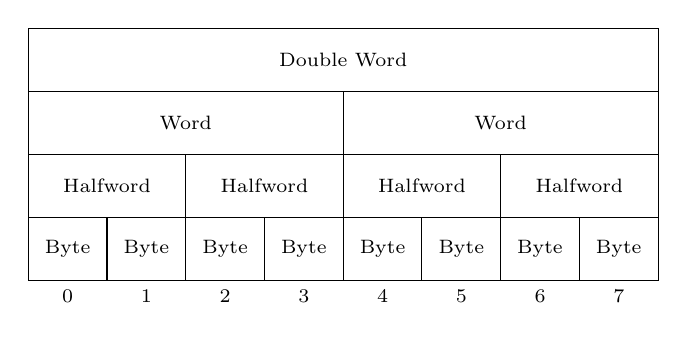
\begin{tikzpicture}[font=\scriptsize]
  \draw (0,0.8) rectangle ++(8,0.8) node[midway]{Double Word};
  \draw (0,0) rectangle ++(4,0.8) node[midway]{Word};
  \draw (4,0) rectangle ++(4,0.8) node[midway]{Word};
  \draw (0,-0.8) rectangle ++(2,0.8) node[midway]{Halfword};
  \draw (2,-0.8) rectangle ++(2,0.8) node[midway]{Halfword};
  \draw (4,-0.8) rectangle ++(2,0.8) node[midway]{Halfword};
  \draw (6,-0.8) rectangle ++(2,0.8) node[midway]{Halfword};
  \foreach \i in {0,...,7}
    \draw (\i,-1.6) rectangle ++(1,0.8) node[midway]{Byte};
  \foreach \i in {0,...,7}
    \node[below] at (\i+0.5,-1.6) {\i};
\end{tikzpicture}
\end{center}

\subsection{IEEE 754 floating point}
\[
  (-1)^S \times (1 + \text{Fraction}) \times 2^{(\text{Exponent} -
  \text{Bias})}
\]
Single precision bias $=127$; double precision bias $=1023$; S.P.\ MAX
exponent field $=255$; D.P.\ MAX exponent field $=2047$.

\begin{center}
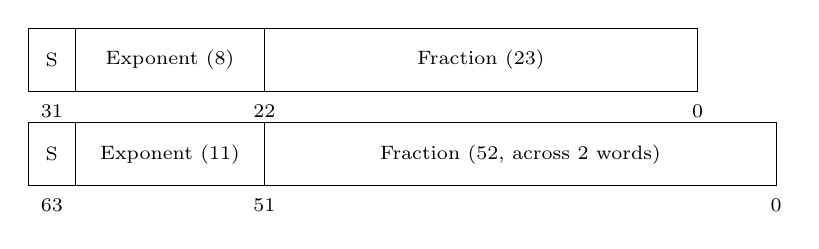
\begin{tikzpicture}[font=\scriptsize]
  \draw (0,0.8) rectangle ++(0.6,0.8) node[midway]{S};
  \draw (0.6,0.8) rectangle ++(2.4,0.8) node[midway]{Exponent (8)};
  \draw (3.0,0.8) rectangle ++(5.5,0.8) node[midway]{Fraction (23)};
  \node[below] at (0.3,0.75) {31};
  \node[below] at (3.0,0.75) {22};
  \node[below] at (8.5,0.75) {0};

  \draw (0,-0.4) rectangle ++(0.6,0.8) node[midway]{S};
  \draw (0.6,-0.4) rectangle ++(2.4,0.8) node[midway]{Exponent (11)};
  \draw (3.0,-0.4) rectangle ++(6.5,0.8) node[midway]{Fraction (52, across 2 words)};
  \node[below] at (0.3,-0.45) {63};
  \node[below] at (3.0,-0.45) {51};
  \node[below] at (9.5,-0.45) {0};
\end{tikzpicture}
\end{center}

\begin{center}
\begin{tabular}{@{}lll@{}}
\toprule
Exponent & Fraction & Object \\
\midrule
0             & 0        & $\pm 0$ \\
0             & $\neq 0$ & $\pm$ Denormalized number \\
1 to MAX$-1$  & anything & $\pm$ Floating-point number \\
MAX           & 0        & $\pm \infty$ \\
MAX           & $\neq 0$ & NaN \\
\bottomrule
\end{tabular}
\end{center}

% ==========================================================================
\section{Exception Handling}

\subsection{Cause and Status registers}
\begin{center}
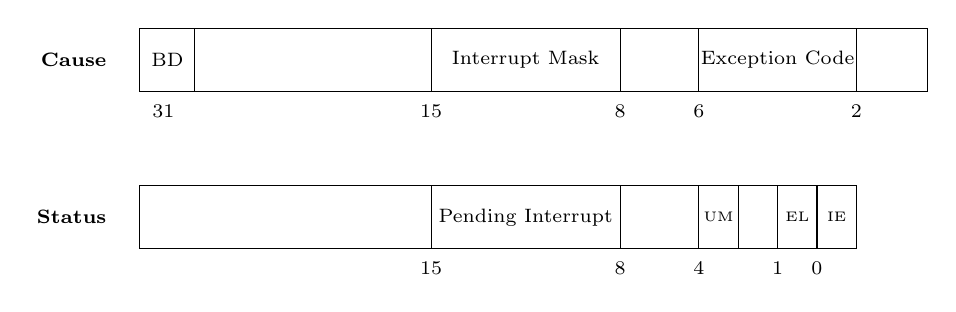
\begin{tikzpicture}[font=\scriptsize]
  \node[left] at (-0.3,2.4) {\textbf{Cause}};
  \draw (0,2.0) rectangle ++(0.7,0.8) node[midway]{BD};
  \draw (0.7,2.0) rectangle ++(3.0,0.8);
  \draw (3.7,2.0) rectangle ++(2.4,0.8) node[midway]{Interrupt Mask};
  \draw (6.1,2.0) rectangle ++(1.0,0.8);
  \draw (7.1,2.0) rectangle ++(2.0,0.8) node[midway]{Exception Code};
  \draw (9.1,2.0) rectangle ++(0.9,0.8);
  \node[below] at (0.3,1.95) {31};
  \node[below] at (3.7,1.95) {15};
  \node[below] at (6.1,1.95) {8};
  \node[below] at (7.1,1.95) {6};
  \node[below] at (9.1,1.95) {2};

  \node[left] at (-0.3,0.4) {\textbf{Status}};
  \draw (0,0.0) rectangle ++(3.7,0.8);
  \draw (3.7,0.0) rectangle ++(2.4,0.8) node[midway]{Pending Interrupt};
  \draw (6.1,0.0) rectangle ++(1.0,0.8);
  \draw (7.1,0.0) rectangle ++(0.5,0.8) node[midway]{\tiny UM};
  \draw (7.6,0.0) rectangle ++(0.5,0.8);
  \draw (8.1,0.0) rectangle ++(0.5,0.8) node[midway]{\tiny EL};
  \draw (8.6,0.0) rectangle ++(0.5,0.8) node[midway]{\tiny IE};
  \node[below] at (3.7,-0.05) {15};
  \node[below] at (6.1,-0.05) {8};
  \node[below] at (7.1,-0.05) {4};
  \node[below] at (8.1,-0.05) {1};
  \node[below] at (8.6,-0.05) {0};
\end{tikzpicture}
\end{center}
BD = Branch Delay, UM = User Mode, EL = Exception Level, IE = Interrupt
Enable.

\subsection{Exception codes}
\begin{center}
\begin{tabular}{@{}clp{5cm}@{}}
\toprule
\# & Name & Cause \\
\midrule
0  & Int   & Interrupt (hardware) \\
4  & AdEL  & Address Error Exception (load or instruction fetch) \\
5  & AdES  & Address Error Exception (store) \\
6  & IBE   & Bus Error on Instruction Fetch \\
7  & DBE   & Bus Error on Load or Store \\
8  & Sys   & Syscall Exception \\
9  & Bp    & Breakpoint Exception \\
10 & RI    & Reserved Instruction Exception \\
11 & CpU   & Coprocessor Unimplemented \\
12 & Ov    & Arithmetic Overflow Exception \\
13 & Tr    & Trap \\
15 & FPE   & Floating Point Exception \\
\bottomrule
\end{tabular}
\end{center}

% ==========================================================================
\section{Opcode \& Funct Field Quick Lookup}

Every instruction table above already lists its \op{opcode/funct} in hex,
which is what you need 95\% of the time (looking up \emph{one} mnemonic's
encoding, or decoding one field you already isolated). The original green
card additionally packs a full 128-row \emph{binary~$\to$~opcode/funct
mnemonic~$\to$~decimal~$\to$~hex~$\to$~ASCII} conversion grid (the card's
own page~3, printed as the left column of \emph{PDF page~2}) -- a
byte-value cross-reference used both for decoding raw instruction words
\emph{and} for looking up ASCII character codes. That grid is already
about as compact as such a table can be; reformatting it here would not
make it more readable, so it is intentionally omitted -- refer to the
original card (\texttt{mips-reference-data.pdf}, PDF page~2, left column,
under ``OPCODES, BASE CONVERSION, ASCII SYMBOLS'') when you need it.

\subsection{Base conversion notes}
\begin{itemize}
  \item opcode(31:26) == 0 $\Rightarrow$ use the funct field (column 1
  above) to find the R-format instruction.
  \item opcode(31:26) == $17_{10}$ ($11_{hex}$) $\Rightarrow$ COP1
  (floating point): if fmt(25:21) == $16_{10}$ ($10_{hex}$), $f=$\op{s}
  (single); if fmt(25:21) == $17_{10}$ ($11_{hex}$), $f=$\op{d} (double).
\end{itemize}

% ==========================================================================
\section{Size Prefixes}
($10^x$ for disk/communication sizes; $2^x$ for memory sizes)

\begin{center}
\begin{tabular}{@{}lll@{}}
\toprule
Prefix & $10^x$ & $2^x$ \\
\midrule
Kilo-  & $10^3$  & $2^{10}$ \\
Mega-  & $10^6$  & $2^{20}$ \\
Giga-  & $10^9$  & $2^{30}$ \\
Tera-  & $10^{12}$ & $2^{40}$ \\
Peta-  & $10^{15}$ & $2^{50}$ \\
Exa-   & $10^{18}$ & $2^{60}$ \\
Zetta- & $10^{21}$ & $2^{70}$ \\
Yotta- & $10^{24}$ & $2^{80}$ \\
\bottomrule
\end{tabular}
\qquad
\begin{tabular}{@{}ll@{}}
\toprule
Prefix & Value \\
\midrule
milli-  & $10^{-3}$ \\
micro-  & $10^{-6}$ \\
nano-   & $10^{-9}$ \\
pico-   & $10^{-12}$ \\
femto-  & $10^{-15}$ \\
atto-   & $10^{-18}$ \\
zepto-  & $10^{-21}$ \\
yocto-  & $10^{-24}$ \\
\bottomrule
\end{tabular}
\end{center}
The symbol for each prefix is just its first letter, except $\mu$ is used
for micro.

\vfill
\noindent\emph{Source: Patterson \& Hennessy, \emph{Computer Organization
and Design}, 4th ed., \textcopyright\ 2009 Elsevier Inc. Content
reorganized for readability; all data reproduced from the original
reference card.}

\end{document}
